\documentclass[letterpaper,10pt]{article}

\usepackage{color}
\usepackage{tikz}
\usepackage{caption}

\setlength{\headheight}{0in}
\setlength{\marginparsep}{0in}
\setlength{\footskip}{0in}
\setlength{\headsep}{0in}
\setlength{\marginparwidth}{0in}
\setlength{\marginparpush}{0in}
\setlength{\voffset}{0in}
\setlength{\hoffset}{-1in}
\setlength{\voffset}{-1in}
\setlength{\oddsidemargin}{0.75in}
\setlength{\evensidemargin}{0.75in}
\setlength{\topmargin}{0.75in}
\setlength{\textheight}{9.5in}
\setlength{\textwidth}{7in}
\setlength{\parindent}{0in}
\setlength{\parskip}{10pt} %change this to match font size

\pagestyle{empty}
\definecolor{gray}{gray}{0.75}
\usetikzlibrary{shapes,arrows,calc}

% define block styles
\tikzstyle{line} = [draw, -latex']
\tikzstyle{block} = [draw, rectangle, text centered, minimum height=2em]
\tikzstyle{mlblock} = [draw, rectangle, text width=10em, text centered, minimum height=2em]
\tikzstyle{decision} = [draw, diamond, text width=4.5em, text centered, node distance=3cm, inner sep=0pt]
\tikzstyle{cloud} = [draw, rectangle, text centered, rounded corners, minimum height=2em]

\begin{document}
    Albert Chang and Nipun Chopra\\
    CSE-380 A6\\
    University at Buffalo\\
    Dr. Kris Schindler\\
    March 8, 2011\\
    \textit{Lab 5 Documentation}

    The objective of Lab 5 was to learn how to use interrupts. The main program
    doesn't really do anything except initialize everything and prompts the user.
    However, with interrupts, the user can enter hexadecimals into the terminal.
    When a valid input is entered, the 7-segment display shows the hexadecimal.
    The user can also push a button to clear the 7-segment display, again
    implemented with an interrupt.

    From the \textit{library.s} file, we imported the following routines:
    \textit{uart\_init}, \textit{output\_character}, \textit{read\_character},
    \textit{output\_string}, and \textit{display\_digit}. Their flowcharts are
    shown in Figs. \ref{flo:uart_init}, \ref{flo:io_character},
    \ref{flo:output_string}, and \ref{flo:display_digit}.

    \begin{figure}[h]
        \begin{center}
    \begin{tikzpicture}[node distance = 3cm, auto]
        \node[cloud] (origin) {Start};
        \node[block, below of=origin, node distance=1.5cm] (enable) {Write 0x5 to PINSEL0 to enable UART0};
        \node[mlblock, below of=enable] (init) {Configure U0LCR:\\%
                                                8-bit word length\\%
                                                1 stop bit\\%
                                                no parity\\%
                                                disable break control\\%
                                                enable access latch};
        \node[block, below of=init] (baud) {Set baud rate to 9600};
        \node[mlblock, below of=baud] (conf) {Configure U0LCR:\\%
                                                8-bit word length\\%
                                                1 stop bit\\%
                                                no parity\\%
                                                disable break control\\%
                                                disable latch access};
        \node[cloud, below of=conf] (stop) {Stop};
        \path[line] (origin) -- (enable);
        \path[line] (enable) -- (init);
        \path[line] (init) -- (baud);
        \path[line] (baud) -- (conf);
        \path[line] (conf) -- (stop);
    \end{tikzpicture}
\end{center}

        \caption{Flowchart of \textit{uart\_init} routine.}
        \label{flo:uart_init}
    \end{figure}

    \begin{figure}[h]
        \begin{minipage}{0.5\linewidth}
            \begin{center}
    \begin{tikzpicture}[node distance = 1.5cm, auto]
        \node[cloud] (origin) {Start};
        \node[decision, below of=origin] (test) {Test THRE in status register};
        \node[block, below of=test, node distance = 3.5cm] (store) {Store byte in transmit register};
        \node[cloud, below of=store] (stop) {Stop};
        \path[line] (origin) -- (test);
        \path[line] (test) -- node [near start] {1} (store);
        \path[line] (test) -| node [near start] {0} +(3,2.25) -- +(0,2.25);
        \path[line] (store) -- (stop);
    \end{tikzpicture}
\end{center}

        \end{minipage}%
        \begin{minipage}{0.5\linewidth}
            \begin{center}
    \begin{tikzpicture}[node distance = 1.5cm, auto]
        \node[cloud] (origin) {Start};
        \node[decision, below of=origin] (test) {Test RDR in status register};
        \node[block, below of=test, node distance = 3.5cm] (read) {Read byte from receive register};
        \node[cloud, below of=read] (stop) {Stop};
        \path[line] (origin) -- (test);
        \path[line] (test) -- node [near start] {1} (read);
        \path[line] (test) -| node [near start] {0} +(3,2) -- +(0,2);
        \path[line] (read) -- (stop);
    \end{tikzpicture}
\end{center}

        \end{minipage}
        \caption{Flowcharts of \textit{output\_character} (left) and \textit{read\_character} (right) routines.}
        \label{flo:io_character}
    \end{figure}

    \begin{figure}[h]
        \begin{center}
    \begin{tikzpicture}[node distance = 1.5cm, auto]
        \node[cloud] (origin) {Start};
        \node[block, below of=origin] (read) {Load byte from memory};
        \node[decision, below of=read] (null) {Is it the null character?};
        \node[cloud, below of=null,node distance=3cm] (stop) {Stop};
        \path[line] (origin) -- (read);
        \path[line] (read) -- (null);
        \path[line] (null) -| node [near start] {no} +(3,3) -- (read);
        \path[line] (null) -- node [near start] {yes} (stop);
    \end{tikzpicture}
\end{center}

        \caption{Flowchart of \textit{output\_string} routine.}
        \label{flo:output_string}
    \end{figure}

    \begin{figure}[h]
        \begin{center}
    \begin{tikzpicture}[node distance = 1.5cm, auto]
        \node[cloud] (origin) {Start};
        \node[block, below of=origin] (clear) {Clear previous display};
        \node[decision, below of=clear] (exit) {Was requested output -1?};
        \node[block, below of=exit, node distance=3cm] (addr) {Get address of lights to be lit};
        \node[block, below of=addr] (display) {Show Display};
        \node[cloud, below of=display] (stop) {Stop};
        \path[line] (origin) -- (clear);
        \path[line] (clear) -- (exit);
        \path[line] (exit) -| node [near start] {yes} +(4,-6) -- (stop);
        \path[line] (exit) -- node [near start] {no} (addr);
        \path[line] (addr) -- (display);
        \path[line] (display) -- (stop);
    \end{tikzpicture}
\end{center}

        \caption{Flowchart of \textit{display\_digit} routine.}
        \label{flo:display_digit}
    \end{figure}

    \clearpage

    The main routine, \textit{lab5} simply calls upon the initialization routines,
    \textit{uart\_init} and \textit{interrupt\_init}, sets up the GPIO, and
    prompts user. After that, it exits. From here on out, everything is handled
    by interrupts. Since even after exiting the program, the microcontroller is
    still running, and can process interrupts, an infinite loop is not necessary.

    \begin{minipage}{\linewidth}
        \begin{center}
    \begin{tikzpicture}[node distance = 1.5cm, auto]
        \node[cloud] (origin) {Start};
        \node[block, below of=origin] (uart) {UART setup};
        \node[block, below of=uart] (ui1) {Get user input 1};
        \node[block, below of=ui1] (val1) {Convert to integer};
        \node[decision, below of=val1] (chck1) {Is it a valid input?};
        \node[block, below of=chck1, node distance=3cm] (ui2) {Get user input 2};
        \node[block, below of=ui2] (val2) {Convert to integer};
        \node[decision, below of=val2] (chck2) {Is it a valid input?};
        \node[block, below of=chck2, node distance=3cm] (format) {Format Output};
        \node[block, below of=format] (mod) {Perform modulo};
        \node[block, below of=mod] (ans) {Convert answer to string};
        \node[block, below of=ans] (output) {Output answer};
        \node[cloud, below of=output] (stop) {Stop};
        \path[line] (origin) -- (uart);
        \path[line] (uart) -- (ui1);
        \path[line] (ui1) -- (val1);
        \path[line] (val1) -- (chck1);
        \path[line] (chck1) -- node [near start] {yes} (ui2);
        \path[line] (chck1) -| node [near start] {no} +(3,4.5) -- (ui1);
        \path[line] (ui2) -- (val2);
        \path[line] (val2) -- (chck2);
        \path[line] (chck2) -- node [near start] {yes} (format);
        \path[line] (chck2) -| node [near start] {no} +(3,4.5) -- (ui2);
        \path[line] (format) -- (mod);
        \path[line] (mod) -- (ans);
        \path[line] (ans) -- (output);
        \path[line] (output) -- (stop);
    \end{tikzpicture}
\end{center}

        \captionof{figure}{Flowchart of \textit{lab5} routine.}
        \label{flo:main}
    \end{minipage}

    The \textit{interrupt\_init} routine sets up all interrupts, which include
    the UART0 interrupt and EINT1 interrupt. For convenience, they are
    classified as fast interrupts. Fig. \ref{flo:interrupt_init} shows how the
    program works.

    \begin{figure}[p]
        \begin{center}
    \begin{tikzpicture}[node distance=1.5cm, auto]
        \node[cloud] (origin) {Start};
        \node[block, below of=origin] (fiq) {Classify as FIQs};
        \node[block, below of=fiq] (enable) {Enable UART0, TIMER0, TIMER1, and EINT1 interrupts};
        \node[block, below of=enable] (uart) {UART0 interrupt on RX};
        \node[block, below of=uart] (timers) {Setup TIMER interrupts};
        \node[block, below of=timers] (eint) {EINT1 interrupts on edge};
        \node[block, below of=eint] (cpsr) {Enable fast interrupts on CPSR};
        \node[cloud, below of=cpsr] (stop) {Stop};
        \path[line] (origin) -- (fiq);
        \path[line] (fiq) -- (enable);
        \path[line] (enable) -- (uart);
        \path[line] (uart) -- (timers);
        \path[line] (timers) -- (eint);
        \path[line] (eint) -- (cpsr);
        \path[line] (cpsr) -- (stop);
    \end{tikzpicture}
\end{center}

        \caption{Flowchart of \textit{interrupt\_init} routine.}
        \label{flo:interrupt_init}
    \end{figure}

    Finally, the interrupt handler, \textit{FIQ\_Handler}, makes up the bulk of
    the code. Nothing is done until there is something to do.

    \begin{minipage}{\linewidth}
        \begin{center}
    \begin{tikzpicture}[node distance=1.5cm, auto]
        \node[cloud] (origin) {Start};
        \node[decision, below of=origin] (timer) {Was the interrupt caused by the timer?};
        \node[block, below of=timer, node distance=3cm] (clear) {Clear interrupt};
        \node[block, below of=clear] (fixed) {Clear terminal and output prompt and top of box};
        \node[block, below of=fixed] (get) {Get position and direction};
        \node[block, below of=get] (updatep) {Update position and change direction if necessary};
        \node[block, below of=updatep] (updatet) {Update terminal output};
        \node[block, below of=updatet] (save) {Save positition and direction};
        \node[block, below of=save] (reset) {Reset TCR and re-enable clock};
        \node[decision, below of=reset] (uart) {Was the interrupt caused by UART?};
        \node[block, below of=uart, node distance=3cm] (input) {Read input};
        \node[block, below of=input] (set) {Adjust speed and direction based on input};
        \node[cloud, below of=set] (stop) {Stop};
        \path[line] (origin) -- (timer);
        \path[line] (timer) -- node [near start] {yes} (clear);
        \path[line] (clear) -- (fixed);
        \path[line] (fixed) -- (get);
        \path[line] (get) -- (updatep);
        \path[line] (updatep) -- (updatet);
        \path[line] (updatet) -- (save);
        \path[line] (save) -- (reset);
        \path[line] (reset) -- (uart);
        \path[line] (uart) -- node [near start] {yes} (input);
        \path[line] (input) -- (set);
        \path[line] (set) -- (stop);
        \path[line] (timer) -| node [near start] {no} +(6,-21) -- (stop);
        \draw (uart) -- node [near start] {no} +(6,0);
    \end{tikzpicture}
\end{center}

        \captionof{figure}{Flowchart of \textit{FIQ\_Handler} routine.}
        \label{flo:fiq_handler}
    \end{minipage}

    There wasn't really a clear distribution of labor, it was programmed in one
    lab session via pair programming.

\end{document}
